\documentclass[10pt,letterpaper]{article}
\usepackage[letterpaper,top=1in,bottom=1in,left=1.05in,right=1.05in]{geometry}
\usepackage[T1]{fontenc}
\usepackage{amsmath,amsthm}
\usepackage{txfonts}
\usepackage[expansion=false]{microtype}
\usepackage{parskip}
\usepackage{tikz}
\usetikzlibrary{arrows.meta,positioning,calc,fit}
\usepackage{booktabs,tabularx,array}
\usepackage{caption}
\usepackage{float}
\usepackage{xcolor}
\usepackage{url}
\usepackage[hidelinks]{hyperref}

\captionsetup{font=small,labelfont=bf,labelsep=period}
\setlength{\parskip}{0.5em}
\linespread{1.03}
\pagestyle{plain}
\emergencystretch=1.5em

\makeatletter
\renewcommand\section{\@startsection{section}{1}{\z@}{-1.3em}{0.45em}{\normalfont\large\bfseries}}
\renewcommand\subsection{\@startsection{subsection}{2}{\z@}{-0.9em}{0.25em}{\normalfont\normalsize\bfseries}}
\renewcommand\thesection{\arabic{section}.}
\renewcommand\thesubsection{\arabic{section}.\arabic{subsection}}
\renewcommand\@seccntformat[1]{\csname the#1\endcsname\ }
\makeatother

\theoremstyle{plain}
\newtheorem{theorem}{Theorem}
\newtheorem{lemma}{Lemma}
\newtheorem{proposition}{Proposition}
\theoremstyle{definition}
\newtheorem{definition}{Definition}

\newcommand{\ak}{\mathsf{ak}}
\newcommand{\ask}{\mathsf{ask}}
\newcommand{\nk}{\mathsf{nk}}
\newcommand{\rivk}{\mathsf{rivk}}
\newcommand{\ivk}{\mathsf{ivk}}
\newcommand{\ovk}{\mathsf{ovk}}
\newcommand{\rk}{\mathsf{rk}}
\newcommand{\fvk}{\mathsf{FVK}}
\newcommand{\Gor}{\mathcal{G}}
\newcommand{\ytilde}{\tilde{y}}
\newcommand{\fn}[1]{\texttt{#1}}
\newcommand{\st}[1]{\textsf{#1}}
\newcommand{\tbd}[1]{\textcolor{red}{[#1]}}

\begin{document}

\begin{center}
{\Large\bfseries Cloakroom: A Dark Pool for Shielded Zcash\\[0.2em] with Scriptless Atomic Settlement}\\[1.1em]
{\normalsize Chris Gachau}\\[0.25em]
{\small October 2026}
\end{center}

\vspace{0.3em}
\begin{quote}
\small
\textbf{Abstract.} Every route out of shielded Zcash today passes through a transparent address
held by an exchange, a bridge or an intent network, which publishes amounts and timing and can
hold funds. Cloakroom trades shielded ZEC against tokens on an EVM chain without either. The two
parties split the spend authorizing key of a fresh Ironwood address into additive shares, and
the counterparty's tokens sit in an escrow whose two exits each publish one share. We give a
timing model with bounded inclusion delay, finality lag and reorganizations, and prove
three things: an honest taker never loses funds and is never held hostage; an honest maker never
loses funds if he comes online once in a stated window, and this condition is necessary; and a
passive observer learns nothing that links the two chains except timing. Model checking the
protocol in TLA$^+$ found that a refund which is included but not yet final can be reorganized
into a theft. This yields a necessary spacing condition between deadlines. Symbolic execution
and invariant testing of the escrow found two issues, both fixed. Measuring 30 days of Zcash
mainnet shows that timing is the binding privacy constraint: without delay a swap transaction
hides among almost no others, and an anonymity set of 50 needs about four hours of randomized
delay, which our wallet implements. The implementation runs end to end on Zcash testnet and
Base Sepolia, and every Zcash transaction it produced was fully shielded.
\end{quote}

\section{Introduction}

Zcash~\cite{zerocash,spec} offers two kinds of value. Transparent value is public, as in
Bitcoin~\cite{bitcoin}. Shielded value is held as encrypted notes, and a fully shielded transaction
shows an observer only that it happened and what fee it paid. Most shielded ZEC is now in
the Ironwood pool introduced by NU6.3 in July 2026~\cite{zip258}.

Shielded value stays private only while it stays shielded. Each crossing between transparent
and shielded value publishes an amount and a time, and matching crossings has linked a large
share of shielded activity to transparent addresses~\cite{kappos,quesnelle,biryukov}; similar
methods recently linked 17.65\% of Railgun withdrawals on Ethereum~\cite{railgun}. On mainnet,
51\% of Ironwood transactions in the last 30 days touched a transparent address
(Section~8.2). Exchange is where this happens: most exchanges withdraw ZEC only to transparent
addresses; NEAR Intents supports ZEC on transparent addresses only~\cite{nearchains}; and Maya
and THORChain hold ZEC in transparent vaults. Each route also adds a custodian. A user reported
a \$589{,}000 payout from a ZEC swap held in a compliance review for more than fifty
days~\cite{freeze}, and on October~1, 2026 NEAR Intents was exploited for about \$3.8 million
before pausing and, according to reports, recovering the funds~\cite{nearexploit}.

Hash-locked atomic swaps~\cite{nolan,herlihy} remove the custodian but need scripts, which
Zcash's shielded pools lack; on transparent outputs, the shared hash links both legs~\cite{xcat}.
Monero, which also lacks scripts, swaps by locking its leg to a key split between the
parties~\cite{gugger,athanor}. Cloakroom brings this approach to Orchard-protocol keys, which the
Ironwood pool uses, and adds what a deployable venue needs. We make five contributions.
\begin{itemize}\setlength\itemsep{0.1em}
\item \textbf{A protocol.} A swap between shielded ZEC and any EVM token whose Zcash leg is
ordinary fully shielded transactions. Claims need Ready and are committed before they are
revealed, payments are pulled, and a punish window removes the hostage case
(Section~4).
\item \textbf{A model and proofs.} A timing model with inclusion delay $D$, finality lag $F$
and reorganizations. Proofs of taker safety without hostage, of maker safety under a liveness
condition, and of the necessity of that condition (Sections~3 and~5).
\item \textbf{Mechanized verification.} A TLA$^+$ model checked by TLC, in which mutations of the
design yield concrete attacks; it produced a necessary deadline-spacing condition. Symbolic
execution, mutation testing, static analysis and stateful fuzzing of the escrow (Section~6).
\item \textbf{A measured privacy analysis.} A simulation argument for passive observers, and
anonymity sets measured on 30 days of Zcash mainnet, which determine the cover-traffic delays our
wallet uses (Section~8).
\item \textbf{An implementation.} Run in thirteen two-party scenarios and on public test networks
(Section~9).
\end{itemize}

We use ``dark pool'' in its trading sense: a venue without pre-trade transparency. Requests and
quotes in Cloakroom travel encrypted, and only the executed price becomes public. Unlike an
exchange-run dark pool, Cloakroom has no central matching; it is bilateral request-for-quote
between a taker and a market maker. The taker is anonymous; the maker's EVM address is public.

\section{Background}

\textbf{Orchard keys.} Orchard~\cite[\S4.2.3]{spec} works over Pallas,
$E_p: y^2 = x^3 + 5$, with prime group order $q$. A spending key yields a spend authorizing key
$\ask \in \mathbb{F}_q^*$, a nullifier key $\nk \in \mathbb{F}_p$ and a randomness
$\rivk \in \mathbb{F}_q$. The spend validating key is $\ak = [\ask]\Gor$, where $\Gor$ is the
RedPallas spend-authorization base point. A full viewing key $(\ak, \nk, \rivk)$ encodes $\ak$
by its $x$-coordinate~\cite[\S5.6.4.4]{spec}, so key generation fixes $\ytilde(\ak)=0$, negating
$\ask$ if needed. From the full viewing key derive the incoming viewing key
$\ivk = \mathsf{Commit}^{\ivk}_{\rivk}(\mathsf{Extract}(\ak),\nk) \notin \{0,\bot\}$, an outgoing
viewing key $\ovk$, and mutually unlinkable diversified addresses.

\textbf{Spending.} A transaction is a set of actions, each pairing a spend and an output. To
spend, one picks a fresh $\alpha$, publishes $\rk = \ak + [\alpha]\Gor$, and signs the ZIP~244
sighash~\cite{zip244} with RedPallas under $\ask + \alpha$. A Halo~2 proof~\cite{halo2} shows
that $\rk$ randomizes the $\ak$ of the spent note's address, that the note is in the commitment
tree, and that the nullifier is correct. An action publishes a value commitment, nullifier,
$\rk$, note commitment, ephemeral key and ciphertexts.

\textbf{Ironwood and NU7.} A soundness flaw in the Orchard action circuit was disclosed in May
2026. NU6.2 (June 2026) fixed the circuit and re-enabled Orchard. NU6.3 (July 28, 2026) then
introduced the Ironwood pool, with its own note-commitment tree, nullifier set and value pool, and
limited the Orchard pool to withdrawals through a turnstile~\cite{zip258}. Ironwood keeps Orchard's keys and addresses, and one incoming
viewing key scans both pools~\cite{zip326}. NU7 (testnet since October~4, 2026) shortens blocks to
25~s and keeps the transaction format~\cite{zip259}. A partially created transaction
(PCZT)~\cite{zip374} separates construction, proving and signing, so that a spend can be signed
by a key that no wallet holds; Zcash's FROST support uses the same interface~\cite{frost,zip312}.

\textbf{The EVM chain.} We use Base, an Ethereum rollup. Its transactions are ordered by a
sequencer; a transaction deposited through the \fn{OptimismPortal} contract on Ethereum must be
included within the sequencing window, 3{,}600 Ethereum blocks or about 12~hours, which still
holds after Base's May 2026 Azul upgrade~\cite{basereliab,opforced}. We measured the lag of
Base's finalized head at 846--890~s on mainnet and 1{,}058--1{,}102~s on Sepolia.

\section{Model and Goals}

\textbf{Parties.} A taker $T$ holds shielded ZEC and wants $u$ tokens; a maker $M$ holds the
tokens. A probabilistic polynomial-time adversary $\mathcal{A}$ statically corrupts at most one of
them. It schedules transactions within the bounds below, observes all public data, and may
crash and later restore the honest party, whose state persists.

\textbf{Time.} Real time is $\tau$; EVM block timestamps satisfy $|ts - \tau| \le \sigma$ and are
monotone.

\textbf{EVM ledger.}
\begin{itemize}\setlength\itemsep{0.05em}
\item \textbf{(E1) Bounded inclusion.} An honest transaction broadcast at $\tau$ is included by
$\tau + D$; if its preconditions fail at inclusion, it reverts.
\item \textbf{(E2) Finality.} At time $\tau$, blocks with timestamp at most $\tau - F$ are final.
Younger blocks may be reorganized, at most $R$ times per swap.
\item \textbf{(E3) Public calldata.} $\mathcal{A}$ learns the calldata of every broadcast
transaction, \emph{including one that later reverts or is reorganized away}.
\end{itemize}

\textbf{Zcash ledger.}
\begin{itemize}\setlength\itemsep{0.05em}
\item \textbf{(Z1) Persistence.} A transaction with $k_Z$ confirmations is reverted with
probability at most $\varepsilon_Z$.
\item \textbf{(Z2) Liveness.} A valid honest transaction is mined within $\Delta_Z$.
\end{itemize}

\textbf{Cryptographic assumptions.}
\begin{itemize}\setlength\itemsep{0.05em}
\item Discrete logarithms are hard on Pallas.
\item Halo~2 is knowledge-sound and zero-knowledge.
\item RedPallas is unforgeable under rerandomized keys~\cite{spec,rerandfrost}.
\item The Fiat--Shamir Schnorr proofs of knowledge are straight-line extractable in the
algebraic group and random oracle models~\cite{agm}.
\item keccak256 and BLAKE2b behave as random oracles.
\item ECDSA on secp256k1 is EUF-CMA.
\item ChaCha20-Poly1305 is IND-CCA, and Gap-DH holds on Pallas.
\item Ironwood shielded transactions with the same number of actions are indistinguishable to an
observer without the keys.
\item Token transfers eventually succeed. A token issuer that blocks an address forever is an
issuer risk, which no protocol over that token can remove.
\end{itemize}

\textbf{Goals.} Let $v$ be the ZEC funded to the joint address and $u$ the tokens escrowed.
\begin{definition}[Taker safety]
An honest $T$ ends in one of three states: (i) she never funded; (ii) she is credited
$u - f_r$, where $f_r$ is the relayer fee; or (iii) she can spend the joint note, or has spent
it. In particular, no execution leaves her ZEC spent by someone else while she is uncredited.
\end{definition}
\begin{definition}[No hostage]
An honest $T$ who funded reaches (ii) or (iii) within bounded time, without any action by $M$.
\end{definition}
\begin{definition}[Maker safety]
An honest $M$ ends either refunded, or with $T$ credited and $M$ able to spend a final joint
note of value at least $v$.
\end{definition}
\begin{definition}[Unlinkability]
A passive observer of both chains cannot distinguish a swap's Zcash transactions from other
Ironwood transactions of the same shape in the same blocks.
\end{definition}

\section{The Protocol}

\subsection{Key setup}
Quotes and requests travel over Zcash memos (Section~7); here we give the keys.
\begin{enumerate}\setlength\itemsep{0.1em}
\item $T$ samples $a \leftarrow \mathbb{F}_q^*$ and a seed $s_T$; $M$ samples $b$ and $s_M$, all fresh
per request. They exchange $A=[a]\Gor$ and $B=[b]\Gor$, each with a Schnorr proof of knowledge.
Each proof's challenge binds the request identifier $\mathsf{sid}$ and the party's role, and each
party verifies the other's proof before use.
\item $T$ commits to $s_T$ in her request and opens it in her acceptance. Both derive
$\nk = H_{\mathbb{F}_p}(\texttt{nk},\mathsf{sid},s_T,s_M)$ and
$\rivk = H_{\mathbb{F}_q}(\texttt{rivk},\mathsf{sid},s_T,s_M)$ with personalized, length-prefixed
BLAKE2b-512.
\item If $\ytilde(A+B)=1$, both parties negate their shares and points. This is deterministic, so
$\ak = A+B$ then has $\ytilde = 0$.
\item Both check that $\fvk_J = (\ak,\nk,\rivk)$ is a valid full viewing key, and derive the
external address at index~0 as $\mathsf{addr}_J$, encoded with an Orchard receiver only. Value
sent there enters Ironwood.
\end{enumerate}
Both parties can view $\mathsf{addr}_J$; spending needs $a+b$. The proofs of knowledge prevent the
rogue-key choice $B = [b']\Gor - A$~\cite{musig}. Our derivation is the
$\mathsf{use\_qsk}=\mathsf{false}$ branch of ZIP~2005~\cite{zip2005}, which Ironwood accepts; joint
notes are therefore not quantum-recoverable. A $\mathsf{use\_qsk}=\mathsf{true}$ variant would derive
$\nk$ and the quantum keys from a jointly agreed secret; no library implements it yet.

\subsection{Escrow}
For each swap the escrow stores the maker, the taker's payout address, the token, $u$, $f_r$, $A$
and $B$, deadlines $t_0 < t_1 < t_2$ and a reveal window $W$. The swap identifier is
$\mathrm{keccak}(\mathit{maker}, \mathit{salt})$, so it is scoped to the maker. The state machine
is in Table~\ref{tab:fsm}.

\begin{table}[H]
\centering\small
\begin{tabularx}{\linewidth}{@{}l l X@{}}
\toprule
\textbf{Call} & \textbf{From} $\to$ \textbf{to} & \textbf{Condition and effect}\\
\midrule
\fn{open} & -- $\to$ \st{Open} & By $M$. $A$ and $B$ on the curve and canonical, $f_r \le u$, $\tau < t_0 < t_1 < t_2$. Pulls $u$ tokens and rejects tokens that deliver less.\\
\fn{setReady} & \st{Open} $\to$ \st{Ready} & By $M$, $\tau < t_0$.\\
\fn{commitClaim} & \st{Ready} $\to$ \st{Locked} & ECDSA signature by the payout key over (escrow, chain id, swap id, $c$, relayer), $\tau < t_1$. Stores $c = \mathrm{keccak}(\mathit{id}, a)$; reveals nothing.\\
\fn{commitClaim} & \st{Open}/\st{Ready} $\to$ \st{Locked} & Same signature, $\tau \ge t_2$ (punish path).\\
\fn{claim}$(a)$ & \st{Locked} $\to$ \st{Claimed} & $\tau < \mathit{lockedAt} + W$, $\mathrm{keccak}(\mathit{id},a)=c$, $[a]\Gor = A$. Credits $u-f_r$ to the payout and $f_r$ to the relayer. No external calls.\\
\fn{refund}$(b)$ & \st{Open} $\to$ \st{Refunded} & $\tau < t_0$, $[b]\Gor = B$. Credits $u$ to $M$. No external calls.\\
\fn{refund}$(b)$ & \st{Open}/\st{Ready} $\to$ \st{Refunded} & $t_1 \le \tau < t_2$.\\
\fn{refund}$(b)$ & \st{Locked} $\to$ \st{Refunded} & $\tau \ge \mathit{lockedAt} + W$.\\
\fn{withdraw} & -- & Anyone; pays an owner's credit. Reveals nothing.\\
\bottomrule
\end{tabularx}
\caption{Escrow state machine. \st{Claimed} and \st{Refunded} are terminal.}
\label{tab:fsm}
\end{table}

The Pallas check uses Jacobian coordinates and a projective comparison with the stored point. It
rejects scalars equal to $0$ or at least $q$, non-canonical coordinates, and the point at
infinity. The escrow verifies a Pallas point directly, so unlike the Monero--Ethereum
construction~\cite{athanor,mrl10} it needs no cross-curve equality proof.

\subsection{Settlement and wallet rules}
\begin{figure}[H]
\centering
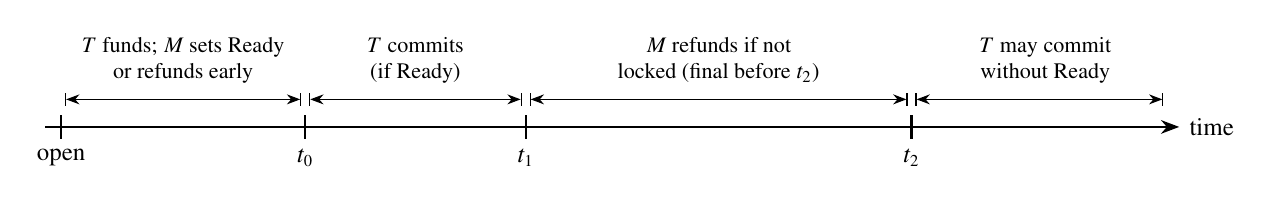
\begin{tikzpicture}[font=\small, >=Stealth]
\draw[thick,->] (0,0) -- (14.4,0) node[right]{time};
\foreach \x/\l in {0.2/open, 3.3/$t_0$, 6.1/$t_1$, 11.0/$t_2$} { \draw[thick] (\x,0.15) -- (\x,-0.15) node[below]{\l}; }
\node[align=center, font=\footnotesize] at (1.75,0.85) {$T$ funds; $M$ sets Ready\\or refunds early};
\node[align=center, font=\footnotesize] at (4.7,0.85) {$T$ commits\\(if Ready)};
\node[align=center, font=\footnotesize] at (8.55,0.85) {$M$ refunds if not\\locked (final before $t_2$)};
\node[align=center, font=\footnotesize] at (12.7,0.85) {$T$ may commit\\without Ready};
\draw[|<->|, thin] (0.25,0.35) -- (3.25,0.35);
\draw[|<->|, thin] (3.35,0.35) -- (6.05,0.35);
\draw[|<->|, thin] (6.15,0.35) -- (10.95,0.35);
\draw[|<->|, thin] (11.05,0.35) -- (14.2,0.35);
\end{tikzpicture}
\caption{Deadlines. After a commit, $T$ reveals within $W$; after $W$, $M$ may refund a lock that was never revealed.}
\end{figure}

\textbf{Happy path.}
\begin{enumerate}\setlength\itemsep{0.1em}
\item $M$ opens the escrow.
\item Once \fn{open} is final, $T$ funds $v + f$ ZEC to $\mathsf{addr}_J$ in a fully shielded
transaction.
\item After $k_Z$ confirmations, $M$ sets Ready.
\item $T$ commits; once the lock is final, she reveals $a$ through a relayer, waits for the claim
to be final, and withdraws.
\item $M$ reads $a$, signs a spend of the joint note under $(a+b)+\alpha$ through PCZT, and sweeps
it to himself with $\ovk = \bot$ and no change to $\mathsf{addr}_J$.
\end{enumerate}
In a refund, $b$ is published and $T$ sweeps the note back the same way.

Table~\ref{tab:rules} lists the wallet rules. They are part of the protocol: the proofs in
Section~5 depend on them, and Section~6 shows that removing each one gives an attack.

\begin{table}[H]
\centering\small
\begin{tabularx}{\linewidth}{@{}l l X@{}}
\toprule
\textbf{Rule} & \textbf{Party} & \textbf{Statement}\\
\midrule
R1 & $T$ & Fund only after \fn{open} is final and every stored parameter equals the quote.\\
R1b & $T$ & Fund only if $M$ can still confirm the note and set Ready before $t_0$.\\
R2c & $T$ & Commit while Ready and before $t_1$, or from $t_2$ if the state is \st{Open} or \st{Ready}. (A late commit reverts and reveals only $c$.)\\
R2r & $T$ & Reveal $a$ only once the lock is final and $\tau + D + F + \mu < \mathit{lockedAt} + W$. Re-send the claim if a reorganization drops it.\\
R3e & $M$ & Refund early only in \st{Open}, near $t_0$, and disjoint from $T$'s funding window.\\
R3d & $M$ & Refund after $t_1$ only if a final block with timestamp $\ge t_1$ shows \st{Open} or \st{Ready}, and $\tau + D + F + \mu < t_2$.\\
R3l & $M$ & Refund a lock only if a final block with timestamp $\ge \mathit{lockedAt}+W$ shows \st{Locked}.\\
R4 & both & All per-request secrets are fresh and are erased at termination.\\
L$_M$ & $M$ & \textbf{Maker liveness:} online at least once in $[t_1 + D + F,\, t_2 - D - F - \mu]$.\\
\bottomrule
\end{tabularx}
\caption{Wallet rules; $\mu$ is a safety margin.}
\label{tab:rules}
\end{table}

\textbf{Parameters.} TLC checks the following conditions; the last one is necessary
(Section~6):
\[
\mu_C \ge D + R F,\quad W \ge F + \mu_C + 1,\quad t_0 - \mathit{open} \ge F + k_Z + D + 1,\quad t_1 - t_0 \ge F + \mu_C,\quad t_2 - t_1 \ge 2D + 2F + \mu + 1,
\]
with all quantities in time units. The maker's software refuses to start with parameters that
violate the last two. Table~\ref{tab:params} gives two deployment profiles for Base mainnet.

\begin{table}[H]
\centering\small
\begin{tabular}{@{}lrr@{}}
\toprule
& \textbf{Live sequencer} & \textbf{Censorship-resistant}\\
\midrule
$D$ (inclusion bound) & 10 min & 12.5 h (forced inclusion)\\
$F$ (finality lag, measured about 15 min) & 20 min & 20 min\\
$k_Z$ & 10 blocks (12.5 min at 75 s) & 10 blocks\\
$t_0 - \mathit{open}$ & 1 h (+ cover delay) & 13.5 h (+ cover delay)\\
$t_1 - t_0$ & 1 h & 13.5 h\\
$W$ & 1.5 h & 14 h\\
$t_2 - t_1$ & 1.2 h + maker downtime tolerance (e.g.\ 24 h) & 26 h + tolerance\\
\bottomrule
\end{tabular}
\caption{Example parameters. The live-sequencer profile assumes the sequencer includes honest transactions within $D$; the censorship-resistant profile assumes only Ethereum-forced inclusion.}
\label{tab:params}
\end{table}

\section{Security Analysis}

\begin{lemma}[Key isolation]
Suppose a corrupted party's share point $X_c$ is accepted with a valid proof of knowledge bound to
$(\mathsf{sid}, \mathit{role})$, and the honest share $x_h$ is never published. Then $\mathcal{A}$
produces a transaction that spends a note at $\mathsf{addr}_J$ with negligible probability.
\end{lemma}
\begin{proof}[Proof sketch]
The reduction $\mathcal{B}$ receives a discrete-logarithm challenge $X_h$ and embeds it as the
honest share. It simulates the honest party's proof of knowledge by programming the random
oracle, and extracts $x_c$ straight-line from $\mathcal{A}$'s proof (algebraic group model), so
that $\ak = X_h + [x_c]\Gor$ with $x_c$ known. Suppose $\mathcal{A}$ outputs a valid spend. By the
knowledge soundness of Halo~2, $\mathcal{B}$ extracts $\alpha$ such that $\rk = \ak + [\alpha]\Gor$.
The spend's RedPallas signature is then a signature under $\rk$, whose discrete logarithm is
$x_h + x_c + \alpha$. Rewinding $\mathcal{A}$ at the random-oracle query that produced the
signature's challenge gives two signatures with the same commitment and different challenges
(forking lemma~\cite{pointcheval}). These yield $\log_{\Gor}\rk$, and hence
$x_h = \log_{\Gor}\rk - x_c - \alpha$. Sign normalization negates $(x_h, x_c)$ together and
preserves the argument. Without the proof of knowledge, $X_c = [x']\Gor - X_h$ gives $\mathcal{A}$
the whole key; this is the rogue-key attack the proof prevents.
\end{proof}

\begin{lemma}[Honest revelations succeed]
(a) A claim sent under R2r becomes final as \st{Claimed}. (b) A refund sent under R3d or R3l
becomes final as \st{Refunded}. (c) Under R3e, a reverted early refund can reveal $b$ only in
\st{Open} before $t_0$.
\end{lemma}
\begin{proof}[Proof sketch]
(a) The lock is final, so no other transition precedes the claim. By E1 and E2 the claim is
included and final before $\mathit{lockedAt}+W$, re-sent at most $R$ times if reorganized. Its
precondition holds, and it makes no external calls, so token behavior cannot make it revert.

(b) For R3d: the final block with timestamp $\ge t_1$ shows no lock. Timestamps are monotone, so
every block before $t_1$ is final and contains no commit. In $[t_1, t_2)$ commits are disabled,
and only $M$ can set Ready. By E1 and E2 the refund is final before $t_2$. A refund that is merely
\emph{included} before $t_2$ could be reorganized past $t_2$; this is the counterexample in
Section~6. For R3l, a final lock past its window can no longer be claimed.

(c) Immediate from R3e.
\end{proof}

\begin{theorem}[Taker safety and no hostage]
Let $T$ be honest, with no assumption on $M$. Except with probability
$\mathsf{negl}+\varepsilon_Z$, the protocol satisfies Definitions~1 and~2. $T$ reaches (ii) or
(iii) by $\max(t_2, \mathit{lockedAt}+W) + 2(D+F) + \Delta_Z$.
\end{theorem}
\begin{proof}[Proof sketch]
By Lemma~1, only someone who knows $a+b$ can spend the joint note. $M$ learns $a$ only from $T$'s
claim, which by Lemma~2(a) credits her (ii). If $M$ refunds, $b$ is public, and $T$ sweeps (iii).
If neither happens by $t_2$, rule R2c lets $T$ commit: refunds from \st{Open} and \st{Ready} are
disabled from $t_2$, so $M$ cannot block the commit, and Lemma~2(a) gives (ii). If $T$ is already
locked, she reveals within $W$. Each step uses only $T$'s own actions.
\end{proof}

\begin{theorem}[Maker safety]
Let $M$ be honest and satisfy L$_M$, with no assumption on $T$. Except with probability
$\mathsf{negl}+\varepsilon_Z$, the protocol satisfies Definition~3.
\end{theorem}
\begin{proof}[Proof sketch]
$T$ is credited only through \st{Locked}, which is reached in one of two ways:
\begin{itemize}\setlength\itemsep{0.05em}
\item \st{Ready} before $t_1$. $M$ sets Ready only after a note of value at least $v+f$ has $k_Z$
confirmations (Z1).
\item $\tau \ge t_2$ from \st{Open} or \st{Ready}. By L$_M$ and Lemma~2(b), $M$'s refund is final
before $t_2$, so this case cannot occur.
\end{itemize}
If $T$ is credited, $M$ knows $a+b$. $T$ does not know $b$: R3d and R3l refunds succeed, so they
end the swap; an R3e leak occurs only before Ready, after which $M$ never sets Ready and refunds
before $t_2$. By Lemma~1 no one else spends the note, and $M$ sweeps it.
\end{proof}

\begin{proposition}[L$_M$ is necessary]
If $M$ is offline throughout $[t_1, t_2)$, a taker who never funds can wait until $t_2$, commit
from \st{Open}, and claim $u$. More generally, any protocol in this model that gives the taker
freedom from hostage, with a scriptless Zcash leg, must let her claim after some deadline
without the maker's cooperation. A maker absent until that deadline therefore cannot be
protected.
\end{proposition}
TLC exhibits the attack (configuration c$'$ in Section~6), and harness scenario s11 executes it
(Section~9). Gugger's punish window~\cite{gugger} has the same requirement.

\begin{theorem}[Liveness]
If both parties are honest and online and the parameter conditions hold, the swap completes by
$t_0 + (t_1 - t_0) + W + 2F + D + \Delta_Z$ after \fn{open}.
\end{theorem}

\textbf{Free options.} After Ready, $T$ may choose not to commit; after committing, she may choose
not to reveal. This is a free option of duration up to $(t_1 - t_{\mathrm{Ready}}) + W$. Before
Ready, $M$ may refund. Han, Lin and Yu model atomic swaps as premium-free American call
options~\cite{optionality}. Cloakroom charges a non-refundable ZEC premium $\pi$ with the taker's
acceptance. An at-the-money option on $u$ with volatility $\sigma$ over time $\theta$ is worth about
$0.4\,\sigma\sqrt{\theta}\,u$. At $\sigma = 100\%$ per year and the live-sequencer profile
($\theta \approx 2.5$~h), that is $0.68\%$ of $u$; at the censorship-resistant profile
($\theta \approx 27.5$~h), $2.2\%$. The premium should cover this plus the maker's \fn{open} and
\fn{refund} gas. The maker's own option before Ready is not priced; it is limited to $t_0$, and an
early refund is public, so it carries a reputational cost.

\section{Mechanized Verification}

\subsection{Protocol model in TLA$^+$}
The model covers:
\begin{itemize}\setlength\itemsep{0.05em}
\item the escrow guards of Table~\ref{tab:fsm};
\item an EVM block history with finality, reorganizations within $F$ and a reorg budget $R$;
\item inclusion within $D$, with reversion when a precondition fails at inclusion;
\item secrets that leak at broadcast, even when the transaction reverts or is reorganized away;
\item a Zcash note that may be reorganized before $k_Z$ confirmations;
\item an adversary that corrupts at most one party and controls scheduling and crashes.
\end{itemize}
Honest parties read only finalized state. We check four invariants:
\begin{itemize}\setlength\itemsep{0.05em}
\item NoDoubleExit;
\item NoFreeClaim (a claim implies a final funding existed);
\item HonestTakerSafe;
\item HonestMakerSafe.
\end{itemize}
We also check two liveness properties under weak fairness: SwapSettles and NoHostage.

\begin{table}[H]
\centering\small
\begin{tabular}{@{}llr@{}}
\toprule
\textbf{Configuration} & \textbf{Result} & \textbf{Distinct states}\\
\midrule
(a) both honest, adversarial scheduling and reorganizations & all invariants hold & 319\\
(b) malicious maker, honest taker & all hold, including HonestTakerSafe & 52{,}423\\
(c) malicious taker, honest maker satisfying L$_M$ & all hold, including HonestMakerSafe & 248{,}853\\
(c$'$) as (c), maker offline in $[t_1,t_2)$ & NoFreeClaim and HonestMakerSafe fail & --\\
liveness, both honest & SwapSettles holds & --\\
liveness, malicious maker & NoHostage holds (punish path) & --\\
\bottomrule
\end{tabular}
\caption{TLC results at $D=F=k_Z=R=1$, $t_0=4$, $t_1=7$, $t_2=13$, $W=4$ (TLC 1.7.4).}
\end{table}

\textbf{Mutations.} We removed one rule at a time; TLC finds a counterexample for each.
\begin{itemize}\setlength\itemsep{0.05em}
\item \emph{Margin too small:} the claim lands after the window and reverts, publishing $a$, and the
taker loses both legs.
\item \emph{Reveal before the lock is final:} a reorganization drops the lock, the claim reverts and
publishes $a$, and the taker loses both legs.
\item \emph{Claim from \st{Open} without Ready} (our first design): free claim.
\item \emph{No punish window:} permanent hostage (liveness failure; the ZEC is locked, not stolen).
\item \emph{$t_2$ too close to $t_1$}, with all rules intact and an online maker (described below).
\item \emph{Refund without finality,} in two variants: a free claim through the punish path.
\end{itemize}

The $t_2$ mutation is the main finding. With $t_2 - t_1 = 4 < 2D+2F+\mu+1 = 6$:
\begin{enumerate}\setlength\itemsep{0.05em}
\item The maker refunds at the earliest moment his rules allow, $t_1 + D + F$.
\item The refund is included but not final at $t_2$.
\item The adversary reorganizes it away, and the escrow is \st{Open} again.
\item A taker who never funded commits through the punish path and claims.
\end{enumerate}
Rule R3d therefore requires the refund to be \emph{final}, not merely included, before $t_2$, and
$t_2 - t_1$ must leave room for that. Our first parameter choice failed this check. The model
also caught a gap in our implementation, which did not re-send a dropped claim; we fixed it. The
model abstracts cryptography to the information each broadcast reveals and checks one small
parameter point; the inequalities are argued in general.

\subsection{The escrow contract}
We verified the final contract in four ways; logs and commands are in the repository's audit
report.
\begin{itemize}\setlength\itemsep{0.1em}
\item \textbf{Symbolic execution (Halmos 0.3.3).} Proved with symbolic arguments, callers, times
and pre-states:
\begin{itemize}\setlength\itemsep{0.05em}
\item each of \fn{open}, \fn{setReady}, \fn{commitClaim}, \fn{claim} and \fn{refund} succeeds if
and only if its guard holds, with exactly the specified effects and credits;
\item every call moves a swap only along the state machine's edges, and terminal states are
absorbing;
\item no claim door and refund door are ever open at the same instant;
\item after $t_2$, an \st{Open} or \st{Ready} swap can be locked but not refunded;
\item swap identifiers are scoped to the maker;
\item \fn{claim} and \fn{refund} make no external calls;
\item state is written before every token call, even when a malicious token re-enters with
arbitrary calldata.
\end{itemize}
Conservation, bounded credits and supply hold after every sequence of up to two calls on any
swaps, up to four calls on one swap, and along a directed six-call claim path. Unrestricted
three-call sequences did not terminate and are not claimed. Four reachability witnesses show the
specifications are not vacuous. Here the curve check is an uninterpreted predicate, so the proofs
hold for any curve arithmetic.
\item \textbf{Curve arithmetic.} The exact source of the Pallas library, with only its constants
replaced, was checked exhaustively on two small prime-order curves with $a=0$ and $Q>P$ (229 and
5{,}023 points). For every scalar $k$ and point $(x,y)$, \fn{isDiscreteLogOf}$(k,x,y)$ holds iff
$0<k<Q$ and $[k]G=(x,y)$. On Pallas itself, test vectors are shared with the Rust implementation
and the group law is fuzzed.
\item \textbf{Mutation testing.} All 22 seeded bugs were caught: guards dropped or loosened, the
punish window moved, effects placed after interactions, each audit fix reverted. Two curve-guard
mutants are beyond symbolic execution and were caught by concrete tests. One of them revealed a
missing test for alias scalars $k+Q$, which we added.
\item \textbf{Stateful fuzzing and static analysis.} Five invariants (conservation, bounded credits,
exclusive and absorbing exits, a per-transition oracle, supply) held over $10^4$ runs of depth 100
each, against the unstubbed contract. Slither 0.11.6 (102 detectors) reported 16 results. One was
ranked high: the balance read before the token pull in \fn{open}. It is not exploitable, because
every re-entrant escrow operation is balance-exact on its own. The rest concern timestamps, log
order and naming.
\item \textbf{Findings, both fixed.} L-01 (low): \fn{open} credited the stated amount, so a
fee-on-transfer token could leave the escrow under-collateralized. \fn{open} now requires the
balance to rise by exactly the amount. I-01 (informational): the Pallas check relied on its caller
for coordinate canonicality. It now checks itself.
\end{itemize}

\begin{table}[H]
\centering\small
\begin{tabular}{@{}lr@{}}
\toprule
\textbf{Transaction} & \textbf{Gas used}\\
\midrule
\fn{open} (two on-curve checks, token pull) & 337{,}254\\
\fn{setReady} & 32{,}494\\
\fn{commitClaim} (signature recovery) & 69{,}456\\
\fn{claim} (scalar check $[a]G=A$) & 555{,}423\\
\fn{refund} (scalar check $[b]G=B$) & 529{,}429\\
\fn{withdraw} & 52{,}259--57{,}071\\
\bottomrule
\end{tabular}
\caption{Gas per transaction from receipts, including intrinsic and calldata cost. The scalar
multiplication dominates \fn{claim} and \fn{refund}.}
\end{table}

\section{Messages}
A maker publishes a unified address, an EVM address and an RFQ public key for the current epoch.
Each message is a 512-byte memo on a zero-value shielded output (ZIP~302 type
\texttt{0xFF}~\cite{zip302}) and is encrypted end to end on top of Zcash's note encryption:
\begin{itemize}\setlength\itemsep{0.05em}
\item the RFQ is encrypted to the epoch key;
\item the Quote and the Accept are encrypted under a Diffie--Hellman exchange of per-request
ephemeral keys, using ChaCha20-Poly1305 with keys derived from BLAKE2b.
\end{itemize}

\begin{table}[H]
\centering\small
\begin{tabularx}{\linewidth}{@{}lXr@{}}
\toprule
\textbf{Message} & \textbf{Encrypted payload} & \textbf{Memo bytes}\\
\midrule
RFQ & id, lots, $A$, $\pi_A$, commitment to $s_T$, payout address, reply address & 269\\
Quote & price, relayer fee, premium, $B$, $\pi_B$, $s_M$, escrow, maker address, $t_0/t_1/t_2/W$ offsets & 281\\
Accept & $s_T$, hash of the quote (sent with the premium as value) & 105\\
\bottomrule
\end{tabularx}
\caption{Messages; only the type, an identifier and ephemeral keys are visible to the recipient's viewing key.}
\end{table}

A quote needs no signature. Only the maker can decrypt the RFQ, so only he knows the fresh reply
address, and the taker checks on chain that the escrow was opened by the maker's EVM address with
the quoted parameters.

\section{Privacy}

\subsection{What each observer learns}
\begin{theorem}[Unlinkability]
Under the assumptions of Section~3, there is a simulator that, given only the swap's public EVM
data ($A$, $B$, $c$, one share, the payout and relayer addresses, $u$, $f_r$ and the times) and
the shapes and block heights of its Zcash transactions, outputs Zcash transactions
indistinguishable from the real ones.
\end{theorem}
\begin{proof}[Proof sketch]
The simulator outputs random Ironwood transactions of the same shapes. Each real spend publishes
$\rk = \ak + [\alpha]\Gor$ for a fresh uniform $\alpha$, which is uniform and independent of $\ak$.
Note commitments are hiding. Nullifiers are pseudorandom under $\nk$, which is never published.
Note ciphertexts reveal nothing without the keys, and Halo~2 proofs are zero-knowledge. A hybrid
argument over these components gives the claim.
\end{proof}
The observer is thus reduced to correlating times, which Section~8.2 measures.

\textbf{Counterparties and infrastructure.}
\begin{itemize}\setlength\itemsep{0.05em}
\item \emph{The maker} learns the requested size, the funding transaction and the taker's fresh
addresses, but not her identity or balances.
\item \emph{The taker} can see that the joint note was spent, since she knows $\nk$, but not where
it went: the sweep uses $\ovk=\bot$. We verified that with the shared $\ovk$ instead, the
counterparty recovers the destination.
\item \emph{The relayer} sees $a$ shortly before it is published.
\item \emph{A light-wallet server} sees the client's address and which full transactions it
fetches. Compact blocks carry no memos, so our wallet fetches each transaction that pays it.
This leak should be closed with Tor and decoy fetches, which we have not implemented.
\end{itemize}

\textbf{Forward secrecy.} An adversary who later obtains a party's viewing key, after the R4
erasure and the epoch-key rotation, learns only the lengths of past messages (Gap-DH and AEAD
security). Before rotation, the epoch key exposes RFQ contents. Our implementation rotates the
epoch key manually.

\textbf{Amounts.} ZEC amounts never appear on chain. The USDC amount is public by design, and lots
of fixed size make the ZEC amount inferable from it. The maker's EVM address links all of his
trades, which is inherent to a public market maker.

\subsection{Measured anonymity sets}
We scanned every Zcash mainnet block from Ironwood's activation to October~14, 2026 through the
public \fn{zec.rocks} lightwalletd server. The primary window is the last 30 days: heights
3{,}483{,}191--3{,}517{,}592 (34{,}402 blocks, mean interval 75.3~s). Cloakroom's transactions
are fully shielded, Ironwood-only and have exactly two actions. This \emph{structural fingerprint}
covers 56{,}361 transactions: 33.1\% of Ironwood transactions, and 68.3\% of Ironwood transactions
have two actions. Compact blocks omit fees and expiry heights. In a sample of 1{,}500 full
transactions of this shape, 92.8\% paid exactly our 10{,}000-zatoshi fee, and 55.7\% also matched
our expiry setting. Expiry height is a wallet fingerprint, and our default of 40 blocks is the
largest group.

\begin{table}[H]
\centering\small
\begin{tabular}{@{}lrrrr@{}}
\toprule
\textbf{Window after a trigger} & \textbf{p10} & \textbf{median} & \textbf{p90} & \textbf{median, full settings}\\
\midrule
same block & 0 & 0 & 4 & 0\\
5 min & 0 & 3 & 14 & 1.9\\
15 min & 3 & 8 & 39 & 5.5\\
60 min & 16 & 33 & 158 & 22.3\\
24 h & 492 & 847 & 4{,}223 & 535\\
\bottomrule
\end{tabular}
\caption{Number of transactions with the structural fingerprint in a window (Zcash mainnet, 30 days). The last column estimates the subset that also matches fee and expiry.}
\end{table}

Without delay, a swap transaction that follows an observable trigger, such as an \fn{open} or a
\fn{claim} on Base, hides among almost no others. Traffic is bursty, averaging 78 matching
transactions per hour but with a median hour of 33, and the first month after activation saw
only 7.3 per hour. Against a delay drawn uniformly from $[0, X]$, an anonymity set of $k=50$ for
90\% of transactions needs $X \approx 175$~min for the structural fingerprint and 240~min for
full settings. For $k = 200$ it needs 615 and 875~min.

\textbf{Cover policy.} Before each Zcash broadcast that follows a public trigger (Quote, Accept,
Fund and the sweeps), the wallet waits for a random delay \emph{and} until at least $k$ matching
transactions have been mined since the trigger, but never past a protocol deadline. Gating on a
count adapts to the burstiness. Because an attacker could inflate the count with its own
look-alike transactions (about 0.02~ZEC for $k=200$), the random minimum delay remains. The
wallet builds each transaction at broadcast time, so its expiry does not reveal the delay. A
private profile with $k=50$ adds about 4~hours to $t_0$ and to the sweeps. This trades capital
lock-up and option value against privacy, and makes the premium correspondingly larger. The RFQ
starts the swap and needs no delay.

\section{Implementation and Evaluation}

\textbf{Implementation.} A Rust node (\fn{orchard}~0.16.0, \fn{pczt}~0.10.0-pre.1,
\fn{zcash\_primitives}~0.31.0-pre.1) implements key setup, messages, maker and taker state
machines, and a light wallet that builds v6 transactions through PCZT and signs joint spends
externally. It syncs from a Zebra node or from a lightwalletd server starting at the server's
Ironwood tree state, and drives the EVM through Foundry's \fn{cast}. Parties persist their state
after every step and can be stopped and restarted at any stage.

\textbf{Against the production verifier.} Against \fn{orchard}~0.16.0 with the current (post-NU6.2) circuit:
\begin{itemize}\setlength\itemsep{0.05em}
\item the joint full viewing key is accepted;
\item a spend signed with one share is rejected;
\item a spend signed with $(a+b)+\alpha$ passes proof, spend-authorization and binding-signature
verification;
\item with $\ovk=\bot$ the counterparty cannot recover the sweep's destination;
\item a rogue share fails its proof of knowledge.
\end{itemize}

\textbf{On a Zebra node.} On Zebra 7.0.0-rc.0 in regtest, a v6 transaction with the real ZIP~244
sighash and an external signature under $(a+b)+\alpha$ was mined. A copy differing only in its
spend signature, made with $b$ alone, was rejected.

\textbf{Two-party scenarios.} Each scenario runs maker and taker as separate processes, which
communicate only through encrypted memos on Zebra regtest and the escrow on a local EVM chain.
Time is advanced on the EVM chain where needed. Balances are checked exactly to the zatoshi, and
every Zcash transaction is read back from the node. On the final code all twelve scenarios pass, with 85 of 85 checks (about 31 minutes in total). Every scenario reads back every Zcash transaction either party made and checks that it is a fully shielded v6 Ironwood transaction with no transparent inputs or outputs. Every scenario also checks that each party that reached a terminal state has erased its per-swap secrets. A party that disappeared mid-swap keeps them, as it must in order to resume.

\begin{table}[H]
\centering\small
\begin{tabularx}{\linewidth}{@{}lXl@{}}
\toprule
& \textbf{Scenario} & \textbf{Observed outcome (checks)}\\
\midrule
s1 & Happy path, with encrypted messages and premium & settled (10/10)\\
s2 & Taker accepts, then disappears before funding & maker refunds before $t_0$, keeps the premium (7/7)\\
s3 & Taker funds, disappears, returns after $t_1$ & R2c declines to commit; maker refunds; taker recovers (8/8)\\
s4 & Maker disappears after \fn{open} & taker completes via the punish path; maker later sweeps (7/7)\\
s5 & Maker sends a rogue key & quote rejected; nothing funded (4/4)\\
s6 & Taker underfunds & no Ready; refund; taker recovers (7/7)\\
s7 & Happy path with NU7 active & settled (10/10)\\
s8 & Unfunded claim while the maker is offline; maker returns in $[t_1,t_2)$ & lock rejected; maker refunds (6/6)\\
s9 & Commit after $t_1$ & reverts revealing only $c$; refund; taker recovers (7/7)\\
s10 & Lock without reveal & maker refunds after $W$; taker recovers (7/7)\\
s11 & Maker offline for all of $[t_1,t_2)$; taker never funds & free claim, as Proposition~1 predicts (6/6)\\
s12 & Cover traffic with $k=4$ & every delayed broadcast waits for $\ge k$ look-alikes (independently counted) (6/6)\\
\bottomrule
\end{tabularx}
\caption{Scenario suite on the final code; every check passed.}
\end{table}

\textbf{Public networks.} On Zcash testnet (NU7 rules) and Base Sepolia, the first version of the
protocol completed one swap and one refund between independent processes. All eleven Zcash
transactions were fully shielded. These runs exposed four problems that local chains did not, all
fixed: a stale nonce, a limit on log queries, crashes on transient errors, and stale balance reads.

\section{Related Work}

\textbf{Hash-locked swaps.} Nolan's construction~\cite{nolan}, formalized by
Herlihy~\cite{herlihy}, and XCAT for Zcash~\cite{xcat} need scripts with hash locks and timelocks.

\textbf{Scriptless swaps.} Gugger's Bitcoin--Monero protocol~\cite{gugger} locks the Monero leg to
a split key and reveals a share through adaptor signatures, with timelocks $t_0$ and $t_1$ and a
punish path; COMIT ran it in production from 2021~\cite{comit}. AthanorLabs replaced the Bitcoin
leg with an Ethereum contract that checks a revealed secp256k1 scalar~\cite{athanor}. Its windows
match those of our first design: claim when ready before its first timeout, or between the
timeouts; refund before the first timeout unless ready, or after the second. Its claims and
refunds are restricted to the respective parties. Ed25519 shares require a cross-group equality
proof~\cite{mrl10}, which a Pallas check avoids. Universal atomic swaps~\cite{uas} need only
signature verification on each chain. Han et al.\ identify the free option of atomic
swaps~\cite{optionality}.

\textbf{Zcash.} Zwap~\cite{zwap} offers Orchard--EVM swaps capped at \$100; forum reviewers
objected that its Orchard-side lock cannot be enforced, since Orchard has no scripts. A grant
proposal for RedPallas adaptor signatures~\cite{zswap} closed without code. Zswap~\cite{zswappets}
is an unrelated scheme for multi-asset swaps within one shielded ledger.

\textbf{Dark pools.} Renegade~\cite{renegade} matches orders at the midpoint with MPC; Penumbra
batches swaps and plans sealed-bid inputs~\cite{penumbra}. Neither settles shielded ZEC.

\section{Limitations}

\begin{itemize}\setlength\itemsep{0.1em}
\item \textbf{Assumptions.} The maker must satisfy L$_M$. Token issuers can freeze credits. A
compromised device exposes the swaps it is running.
\item \textbf{Privacy.} Timing is the binding constraint, and cover delays cost hours. The light
wallet leaks its fetches to the server. The maker is public.
\item \textbf{Verification scope.} The TLA$^+$ model checks one small parameter point and abstracts
cryptography. Halmos proves bounded call sequences. The contracts have not had an external audit.
\item \textbf{Implementation.} One maker per request; manual epoch-key rotation; no Tor;
cover-delay waits block the maker's other swaps; the relayer is trusted for liveness only.
\item \textbf{Not tested.} Forced inclusion through Ethereum, mainnet deployments, and production
window lengths.
\end{itemize}

\section{Conclusion}

Cloakroom settles trades between shielded ZEC and EVM tokens without custodians and without
leaving the shielded pool. Its safety does not rest on tests alone. Proofs give it under explicit
timing assumptions. A model checker shows that each rule is needed, and found a reorganization
attack in a natural parameter choice. Symbolic execution covers the contract. Its privacy has been
measured on mainnet rather than assumed: shielding hides amounts and parties completely, and
timing is what remains, which the wallet addresses with count-gated delays.

\renewcommand{\refname}{References}
\begin{thebibliography}{99}\small\setlength\itemsep{0.05em}
\bibitem{zerocash} E. Ben-Sasson, A. Chiesa, C. Garman, M. Green, I. Miers, E. Tromer, M. Virza, ``Zerocash: Decentralized anonymous payments from Bitcoin,'' \emph{IEEE S\&P}, 2014.
\bibitem{spec} D. Hopwood, S. Bowe, T. Hornby, N. Wilcox, ``Zcash Protocol Specification,'' v2026.7.0, \url{https://zips.z.cash/protocol/protocol.pdf}.
\bibitem{bitcoin} S. Nakamoto, ``Bitcoin: A peer-to-peer electronic cash system,'' 2008.
\bibitem{zip258} D. Hopwood, ``ZIP 258: Deployment of the NU6.3 network upgrade,'' \url{https://zips.z.cash/zip-0258}.
\bibitem{zip326} D. Hopwood, ``ZIP 326: NU6.3 consequences for wallets,'' \url{https://zips.z.cash/zip-0326}.
\bibitem{zip2005} D. Hopwood, J. Grigg, ``ZIP 2005: Ironwood quantum recoverability,'' \url{https://zips.z.cash/zip-2005}.
\bibitem{zip259} D. Ojha, ``ZIP 259: Deployment of the NU7 network upgrade,'' \url{https://zips.z.cash/zip-0259}.
\bibitem{zip244} K. Nuttycombe, D. Hopwood, J. Grigg, ``ZIP 244: Transaction identifier non-malleability,'' \url{https://zips.z.cash/zip-0244}.
\bibitem{zip374} J. Grigg, ``ZIP 374: Partially created Zcash transaction format,'' \url{https://zips.z.cash/zip-0374}.
\bibitem{zip312} C. Gouv\^{e}a, C. Komlo, D. Connolly, ``ZIP 312: FROST for spend authorization multisignatures,'' \url{https://zips.z.cash/zip-0312}.
\bibitem{zip302} J. Graber, J. Grigg, ``ZIP 302: Standardized memo field format,'' \url{https://zips.z.cash/zip-0302}.
\bibitem{halo2} Electric Coin Company, ``The halo2 book,'' \url{https://zcash.github.io/halo2/}; S. Bowe, J. Grigg, D. Hopwood, ``Recursive proof composition without a trusted setup,'' IACR ePrint 2019/1021.
\bibitem{frost} C. Komlo, I. Goldberg, ``FROST: Flexible round-optimized Schnorr threshold signatures,'' \emph{SAC}, 2020.
\bibitem{rerandfrost} C. Gouv\^{e}a, C. Komlo, ``Re-randomized FROST,'' IACR ePrint 2024/436.
\bibitem{agm} G. Fuchsbauer, E. Kiltz, J. Loss, ``The algebraic group model and its applications,'' \emph{CRYPTO}, 2018.
\bibitem{pointcheval} D. Pointcheval, J. Stern, ``Security arguments for digital signatures and blind signatures,'' \emph{J. Cryptology} 13(3), 2000.
\bibitem{musig} G. Maxwell, A. Poelstra, Y. Seurin, P. Wuille, ``Simple Schnorr multi-signatures with applications to Bitcoin,'' \emph{Designs, Codes and Cryptography}, 2019.
\bibitem{kappos} G. Kappos, H. Yousaf, M. Maller, S. Meiklejohn, ``An empirical analysis of anonymity in Zcash,'' \emph{USENIX Security}, 2018.
\bibitem{quesnelle} J. Quesnelle, ``On the linkability of Zcash transactions,'' arXiv:1712.01210, 2017.
\bibitem{biryukov} A. Biryukov, D. Feher, ``Privacy and linkability of mining in Zcash,'' \emph{IEEE CNS}, 2019.
\bibitem{railgun} K. Huseynov, A. Shahzaib, I. A. Seres, J. Tapolcai, ``A tattered cloak of invisibility: Measuring anonymity loss in Railgun on Ethereum,'' arXiv:2606.25926, 2026.
\bibitem{nearchains} NEAR Intents, ``Supported chains,'' \url{https://docs.near-intents.org/resources/chain-support}.
\bibitem{freeze} C. Monasterio, ``\$589K USDT stuck for 50 days after Zodl swap,'' Crypto Economy, Sep.\ 11, 2026 (a user report).
\bibitem{nearexploit} The Block, ``NEAR Intents halts services after \$3.8 million exploit,'' Oct.\ 1, 2026; Crypto Briefing, ``NEAR Intents recovers exploit funds,'' Oct.\ 2026.
\bibitem{nolan} T. Nolan, ``Alt chains and atomic transfers,'' bitcointalk.org, 2013.
\bibitem{herlihy} M. Herlihy, ``Atomic cross-chain swaps,'' \emph{PODC}, 2018.
\bibitem{xcat} J. Graber, ``ZIP 300: Cross-chain atomic transactions,'' \url{https://zips.z.cash/zip-0300}, 2017.
\bibitem{gugger} J. Gugger, ``Bitcoin--Monero cross-chain atomic swap,'' IACR ePrint 2020/1126.
\bibitem{comit} COMIT, ``xmr-btc-swap,'' \url{https://github.com/comit-network/xmr-btc-swap}; continued as eigenwallet.
\bibitem{athanor} E. Binks, ``Cross-chain atomic swaps between Ethereum and Monero,'' AthanorLabs, 2022; contract \fn{SwapCreator.sol}, \url{https://github.com/AthanorLabs/atomic-swap}.
\bibitem{mrl10} S. Noether, ``Discrete logarithm equality across groups,'' MRL-0010, 2018.
\bibitem{uas} S. A. K. Thyagarajan, G. Malavolta, P. Moreno-Sanchez, ``Universal atomic swaps: Secure exchange of coins across all blockchains,'' \emph{IEEE S\&P}, 2022.
\bibitem{optionality} R. Han, H. Lin, J. Yu, ``On the optionality and fairness of atomic swaps,'' \emph{ACM AFT}, 2019; IACR ePrint 2019/896.
\bibitem{zswappets} F. Engelmann, T. Kerber, M. Kohlweiss, M. Volkhov, ``Zswap: zk-SNARK based non-interactive multi-asset swaps,'' \emph{PoPETs} 2022(4).
\bibitem{zwap} Atheon, ``Zwap: Trustless shielded atomic swaps for Zcash (early access),'' Zcash Community Forum, May 2026, \url{https://forum.zcashcommunity.com/t/zwap-trustless-shielded-atomic-swaps-for-zcash-early-access/55874}.
\bibitem{zswap} Stallion Labs, ``Grant application: zswap,'' Zcash Community Grants issue \#443, Sep.\ 2026.
\bibitem{renegade} Renegade, documentation, \url{https://docs.renegade.fi}.
\bibitem{penumbra} Penumbra, ``Decentralized exchange,'' \url{https://protocol.penumbra.zone/main/dex.html}.
\bibitem{basereliab} Base, ``Reliability and liveness,'' \url{https://docs.base.org/specifications/security/reliability-and-liveness}.
\bibitem{opforced} Optimism, ``Forced transaction,'' \url{https://docs.optimism.io/stack/transactions/forced-transaction}.
\end{thebibliography}

\appendix
\section*{Appendix: Test Vectors}
{\small
$\Gor$ (from \fn{orchard}~0.16.0):\\
\texttt{x = 0x375523b328f1d6063b8d187c3e5f445f0c7f0ce37b70a10c8d1a7284b875c963}\\
\texttt{y = 0x1ad0357fdf1a66db7b10bcfcfed624fbdfc914fec005bdd84ce33e817b0c3bc9}

A share $a$ and $A = [a]\Gor$:\\
\texttt{a\ \ \ = 0x195661e2e4789b7f57137b2e777736d79720270638d12e4882fd95e52a73d6b3}\\
\texttt{A.x = 0x17a182b1eb9594581ecaad0fcb61546f4c366cc57b9575ddde22ca56963c304c}\\
\texttt{A.y = 0x19b252972f768cc5708b251baca77a9afd02dddd9531510aafb13c4824d7b61f}
}

\end{document}
